\section{Charakterystyka środowiska sprzętowego NVIDIA CUDA i modelu wykonania SIMT}

\subsection{Wprowadzenie}
CUDA (Compute Unified Device Architecture) to opracowana przez firmę NVIDIA platforma umożliwiająca wykorzystanie procesorów graficznych (GPU) do obliczeń równoległych. Środowisko sprzętowe CUDA charakteryzuje się specyficzną architekturą opartą na modelu równoległego wykonywania instrukcji SIMT (\textit{Single Instruction Multiple Threads}).

\subsection{Architektura sprzętowa NVIDIA CUDA}

Architektura sprzętowa CUDA opiera się na hierarchicznej organizacji zasobów obliczeniowych:
\begin{itemize}
    \item \textbf{GPU (Graphics Processing Unit)} – jednostka obliczeniowa zawierająca wiele multiprocesorów strumieniowych.
    \item \textbf{Multiprocesory strumieniowe (SM – Streaming Multiprocessor)} – podstawowe jednostki obliczeniowe GPU, zawierające zestawy rdzeni.
    \item \textbf{Rdzenie CUDA (CUDA Cores)} – elementarne jednostki wykonawcze realizujące operacje arytmetyczne i logiczne.
    \item \textbf{Warp} – grupa 32 wątków wykonywanych równocześnie w jednym SM.
    \item \textbf{Blok wątków (Thread Block)} – zestaw wątków współdzielących pamięć lokalną.
    \item \textbf{Siatka bloków (Grid of Blocks)} – zbiór bloków realizujących obliczenia w danym kernelu CUDA.
\end{itemize}

\begin{figure}[h]
    \centering
    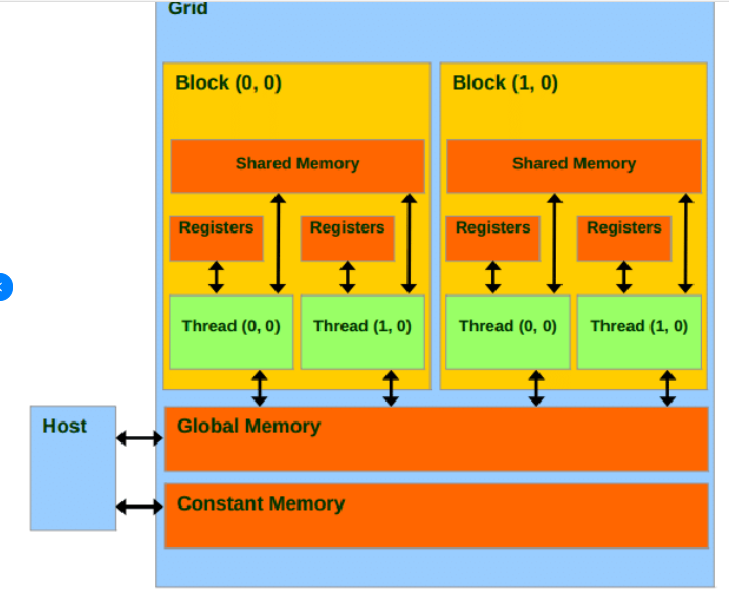
\includegraphics[width=0.7\textwidth]{cuda_architecture.png}
    \caption{Hierarchiczna organizacja zasobów CUDA.}
\end{figure}

\subsection{Model wykonania SIMT (Single Instruction Multiple Threads)}

Model \textbf{SIMT} stosowany w architekturze CUDA polega na jednoczesnym wykonywaniu tej samej instrukcji przez wiele wątków.

\textbf{Cechy SIMT:}
\begin{itemize}
    \item Każdy multiprocesor SM wykonuje wiele wątków równocześnie.
    \item Wątki w ramach jednego warpa (32 wątki) wykonują te same instrukcje, ale na różnych danych.
    \item Gdy występuje rozgałęzienie warunkowe, wątki w warpie mogą wykonywać różne ścieżki kodu (\textit{thread divergence}), co prowadzi do spadku wydajności.
\end{itemize}

\subsection{Struktura wykonania w CUDA}

\subsubsection{1. Hierarchia wątków w modelu CUDA}
\begin{itemize}
    \item \textbf{Wątek (Thread)} – jednostka wykonawcza pracująca na określonych danych.
    \item \textbf{Blok wątków (Thread Block)} – grupa wątków, które mogą współdzielić pamięć współdzieloną.
    \item \textbf{Siatka bloków (Grid of Blocks)} – zestaw bloków, które wykonują równoległe obliczenia.
\end{itemize}

\textbf{Przykład konfiguracji siatki i bloków:}
\begin{verbatim}
kernel<<<numBlocks, threadsPerBlock>>>(d_data);
\end{verbatim}

\subsubsection{2. Organizacja pamięci w CUDA}
CUDA udostępnia różne rodzaje pamięci:
\begin{itemize}
    \item \textbf{Pamięć rejestrów} – najszybsza, ale ograniczona ilościowo.
    \item \textbf{Pamięć współdzielona (Shared Memory)} – szybka pamięć dostępna w obrębie jednego bloku wątków.
    \item \textbf{Pamięć globalna (Global Memory)} – dostępna dla wszystkich wątków, ale o dużym opóźnieniu.
    \item \textbf{Pamięć stała (Constant Memory)} – zoptymalizowana dla niezmiennych danych.
    \item \textbf{Pamięć tekstur i powierzchni (Texture \& Surface Memory)} – wykorzystywana w operacjach graficznych i analizie obrazu.
\end{itemize}

\subsection{Przykładowa implementacja kernela CUDA}
Przykład prostego kernela sumującego dwa wektory:
\begin{verbatim}
__global__ void addVectors(int *a, int *b, int *c, int n) {
    int idx = threadIdx.x + blockIdx.x * blockDim.x;
    if (idx < n) {
        c[idx] = a[idx] + b[idx];
    }
}
\end{verbatim}

\subsection{Zalety i ograniczenia modelu SIMT}

\textbf{Zalety:}
\begin{itemize}
    \item Wysoka wydajność w obliczeniach masowo-równoległych.
    \item Efektywne wykorzystanie zasobów sprzętowych GPU.
    \item Redukcja czasu obliczeń w porównaniu do CPU.
\end{itemize}

\textbf{Ograniczenia:}
\begin{itemize}
    \item Problemy z \textit{thread divergence}, gdy wątki wykonują różne ścieżki kodu.
    \item Konieczność optymalizacji dostępu do pamięci globalnej.
    \item Wysokie wymagania pamięciowe przy dużych rozmiarach danych.
\end{itemize}

\subsection{Podsumowanie}
\begin{itemize}
    \item CUDA pozwala na programowanie GPU z wykorzystaniem hierarchii wątków.
    \item Model SIMT umożliwia jednoczesne wykonywanie tej samej instrukcji przez wiele wątków.
    \item Optymalizacja pamięci i unikanie \textit{thread divergence} są kluczowe dla efektywnego programowania CUDA.
    \item CUDA znajduje zastosowanie w obliczeniach naukowych, sztucznej inteligencji i grafice komputerowej.
\end{itemize}
